\chapter{Resultados}
\label{cap:resultados}

Este capítulo apresenta o sistema desenvolvido e os resultados dos experimentos descritos na \autoref{sec:protocolo}.

\section{Levantamento de requisitos e modelagem}

Por meio de reuniões com os membros e professores da LORD-UEPG, foram catalogadas as principais restrições e necessidades do acompanhamento de DTM e próteses e mapeado o fluxo de atendimento. A análise da ficha resultou na classificação apresentada no \autoref{qua:ficha-captacao} e no esquema JSON da ficha inicial, com 144 campos distribuídos em 15 seções. Todas as questões numeradas da ficha em papel (1 a 75, exceto a 43, que é a legenda da escala de palpação) e os blocos não numerados (queixa principal, condição DTM, características relatadas, Eixo~I, tecidos moles, condição periodontal, observações e plano de tratamento) estão representados, o que é verificado por um teste automatizado de cobertura.

A \autoref{tb:campos-captacao} resume os campos por forma de captação. Os 15 campos de decisão clínica são exclusivamente humanos. Os 26 campos do questionário de dor, que incluem as escalas da GCPS, admitem apenas o formulário, de modo que a IA não pode atribuir notas de dor. Os demais 103 campos admitem ditado e podem receber sugestões, sempre sujeitas à revisão humana. Além da ficha inicial, foram definidos os esquemas da ficha de retorno (proposta a validar com a Liga), do odontograma, na notação FDI, e dos dados cadastrais do paciente. Estes últimos ficam separados dos dados clínicos, e os campos identificadores são marcados para armazenamento cifrado.

\begin{table}[htbp]
	\caption{Campos da ficha inicial por forma de captação}
	\label{tb:campos-captacao}
	\footnotesize
	\centering
	\begin{tabular}{|l|c|c|}
		\hline
		\textbf{Forma de captação} & \textbf{Seções} & \textbf{Campos} \\ \hline
		Exclusivamente humana & 4 & 15 \\ \hline
		Somente formulário & 1 & 26 \\ \hline
		Formulário, componentes visuais ou ditado com IA & 10 & 103 \\ \hline
		\textbf{Total} & \textbf{15} & \textbf{144} \\ \hline
	\end{tabular}
	\fonte{Os autores (2026).}
\end{table}

A partir desse esquema, foi construído o modelo de dados híbrido da \autoref{fig:der}, que prioriza campos numéricos e categóricos estruturados para viabilizar o acoplamento das ferramentas de análise em Python e Pandas.

\section{Sistema desenvolvido}

A interface foi implementada em React e consome exclusivamente a API. As telas foram capturadas automaticamente por um roteiro do Playwright executado sobre o ambiente de desenvolvimento com dados sintéticos, o que torna as figuras reprodutíveis a cada versão do sistema.

A tela do paciente (\autoref{fig:tela-paciente}) reúne os atendimentos, com o status e a completude de cada ficha, os dados pessoais (decifrados apenas para quem tem acesso), os tratamentos e os consentimentos. Quando não há TCLE registrado, a tela o sinaliza antes da abertura de um atendimento (RF02, RF03).

\begin{figure}[htbp]
	\caption{Tela do paciente}
	\label{fig:tela-paciente}
	\centering
	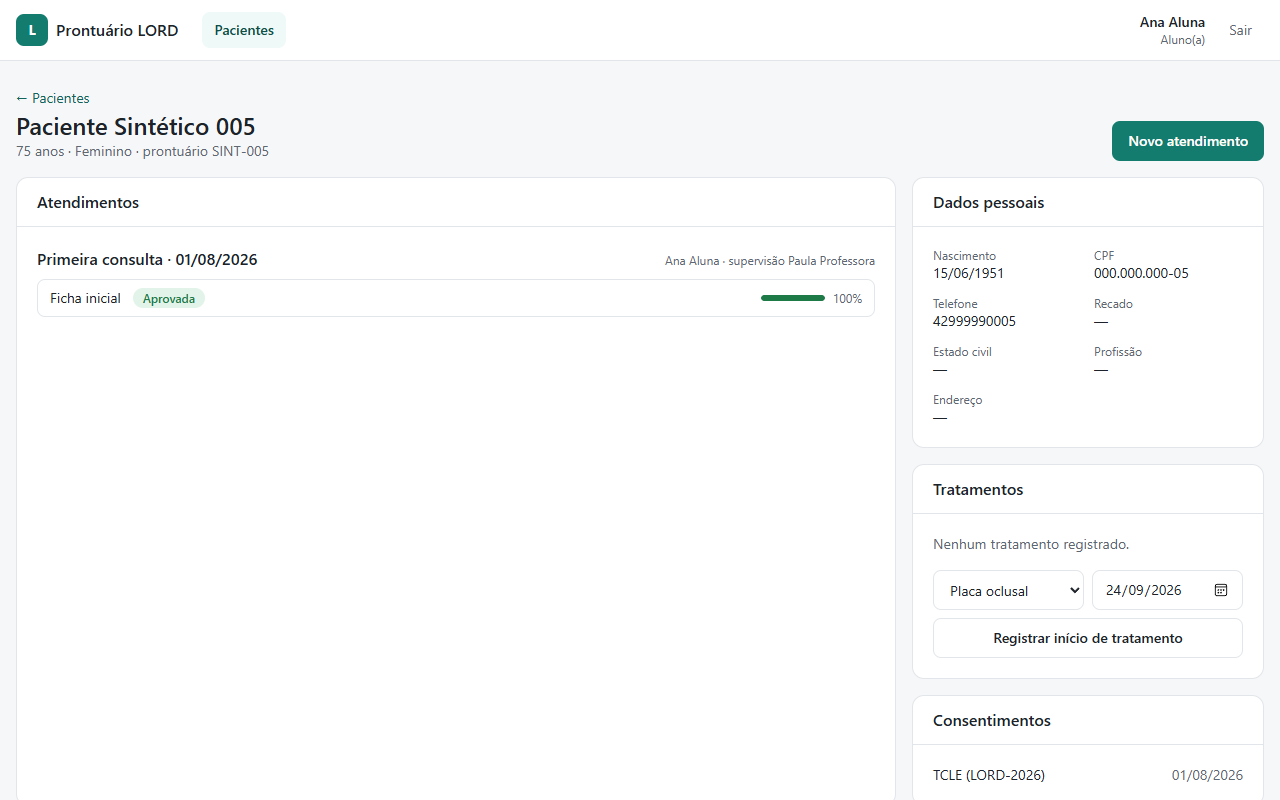
\includegraphics[width=\textwidth]{figuras/03-paciente}
	\fonte{Os autores (2026), com dados sintéticos.}
\end{figure}

O editor da ficha (\autoref{fig:tela-anamnese}) é gerado inteiramente a partir do esquema JSON: cada seção da ficha em papel aparece na navegação lateral com a contagem de campos preenchidos, e cada campo recebe o controle adequado ao seu tipo. Listas de opções viram botões, respostas sim/não viram um par de botões, as escalas de 0 a 10 viram uma régua colorida, e medidas em milímetros viram campos numéricos. O número da questão no papel acompanha cada campo, o que facilita a transição dos alunos habituados à ficha impressa. Campos condicionais, como os medicamentos em uso, só aparecem quando a resposta de controle os torna aplicáveis, e o valor é descartado se a resposta mudar. A validação ocorre no próprio navegador, com o mesmo esquema e as mesmas mensagens usados pela API.

\begin{figure}[htbp]
	\caption{Editor da ficha: seção de história médica}
	\label{fig:tela-anamnese}
	\centering
	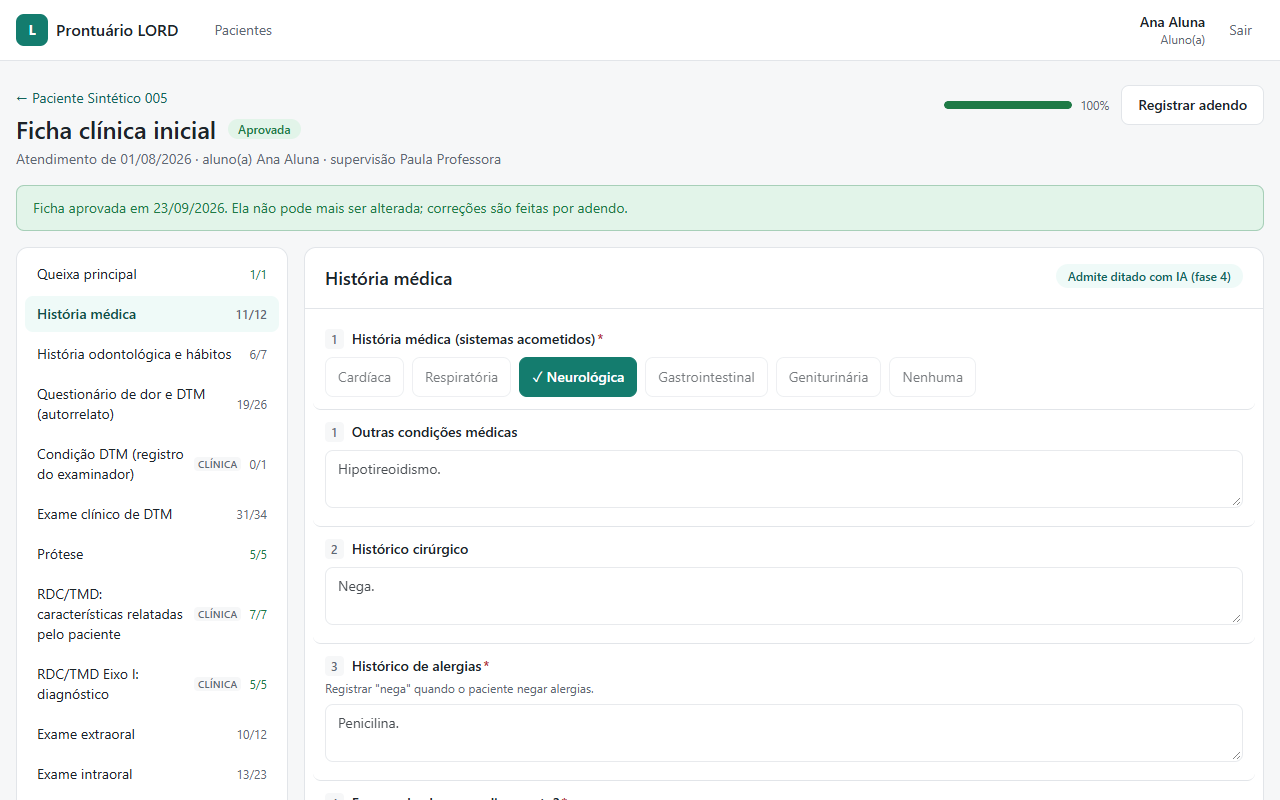
\includegraphics[width=\textwidth]{figuras/04-ficha-historia-medica}
	\fonte{Os autores (2026), com dados sintéticos.}
\end{figure}

A palpação muscular e articular (questões 43 a 45) é registrada em um mapa facial esquemático (\autoref{fig:tela-palpacao}), no qual cada sítio muda de cor conforme a intensidade de 0 a 3. Ao lado há uma tabela equivalente, mais precisa ao toque e acessível por teclado. O odontograma (\autoref{fig:tela-odontograma}) segue a numeração FDI. Cada dente tem cinco faces clicáveis, marcadas segundo a ferramenta escolhida, e a face mesial fica sempre voltada para a linha média. Ao selecionar um dente, é possível registrar sua ausência e condições como tratamento endodôntico ou recessão (RF04).

\begin{figure}[htbp]
	\caption{Mapa de palpação muscular e articular}
	\label{fig:tela-palpacao}
	\centering
	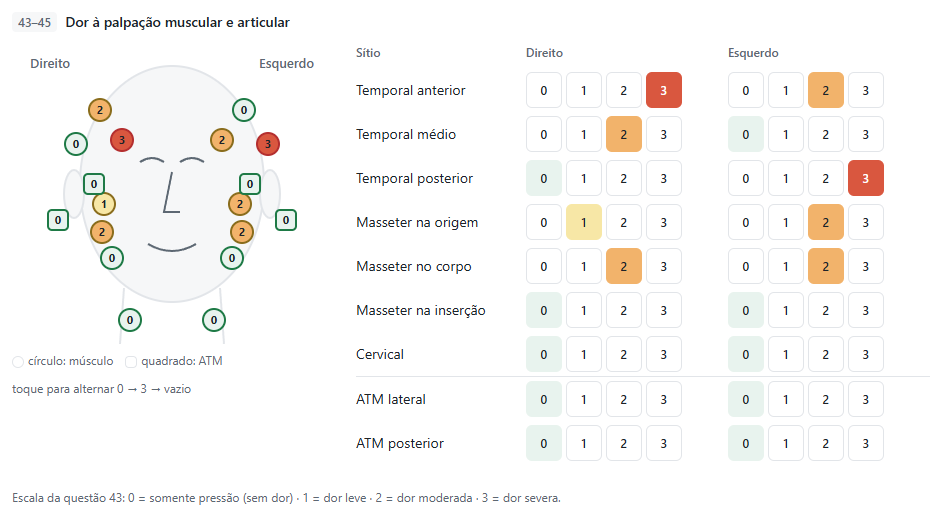
\includegraphics[width=\textwidth]{figuras/06-mapa-palpacao}
	\fonte{Os autores (2026), com dados sintéticos.}
\end{figure}
\begin{figure}[htbp]
	\caption{Odontograma com marcações de exemplo}
	\label{fig:tela-odontograma}
	\centering
	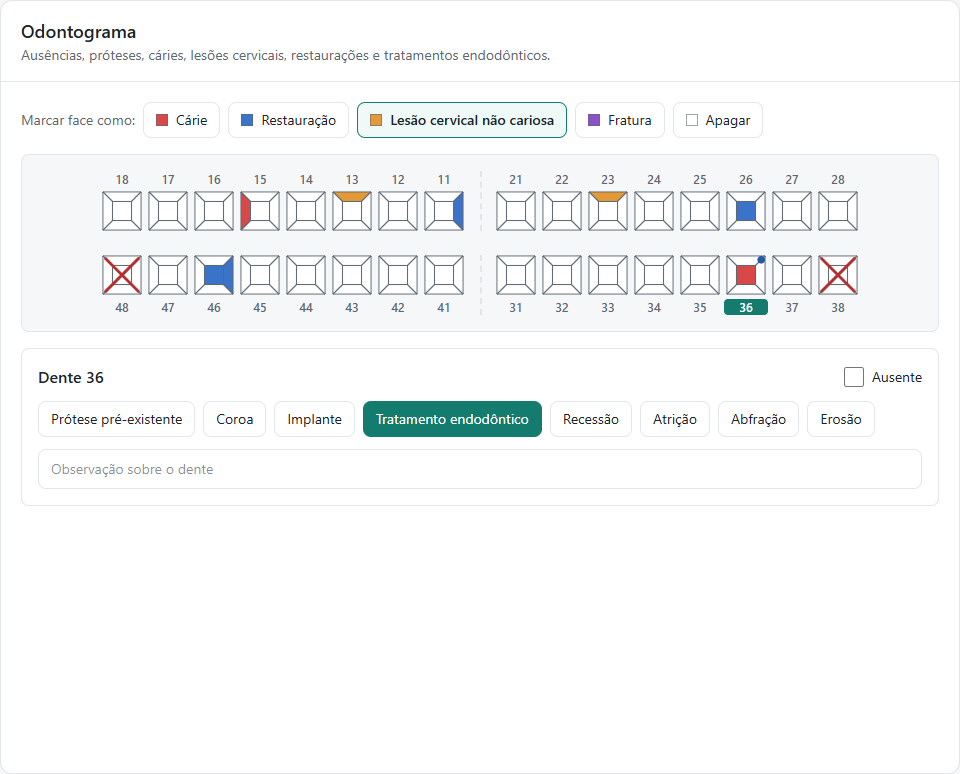
\includegraphics[width=\textwidth]{figuras/08-odontograma}
	\fonte{Os autores (2026), com dados sintéticos.}
\end{figure}

As seções de decisão clínica são identificadas na navegação e no cabeçalho da seção como exclusivas do examinador (\autoref{fig:tela-diagnostico}), reforçando para o usuário a restrição que o esquema impõe ao módulo de IA. O professor acompanha as fichas enviadas pelos alunos em uma fila de revisão (\autoref{fig:tela-revisao}) e, ao abrir cada uma, pode devolvê-la com um comentário ou aprová-la (RF05). Após a aprovação, a ficha é exibida somente para leitura, com a opção de registrar um adendo (RF06).

\begin{figure}[htbp]
	\caption{Seção de diagnóstico, exclusiva do examinador}
	\label{fig:tela-diagnostico}
	\centering
	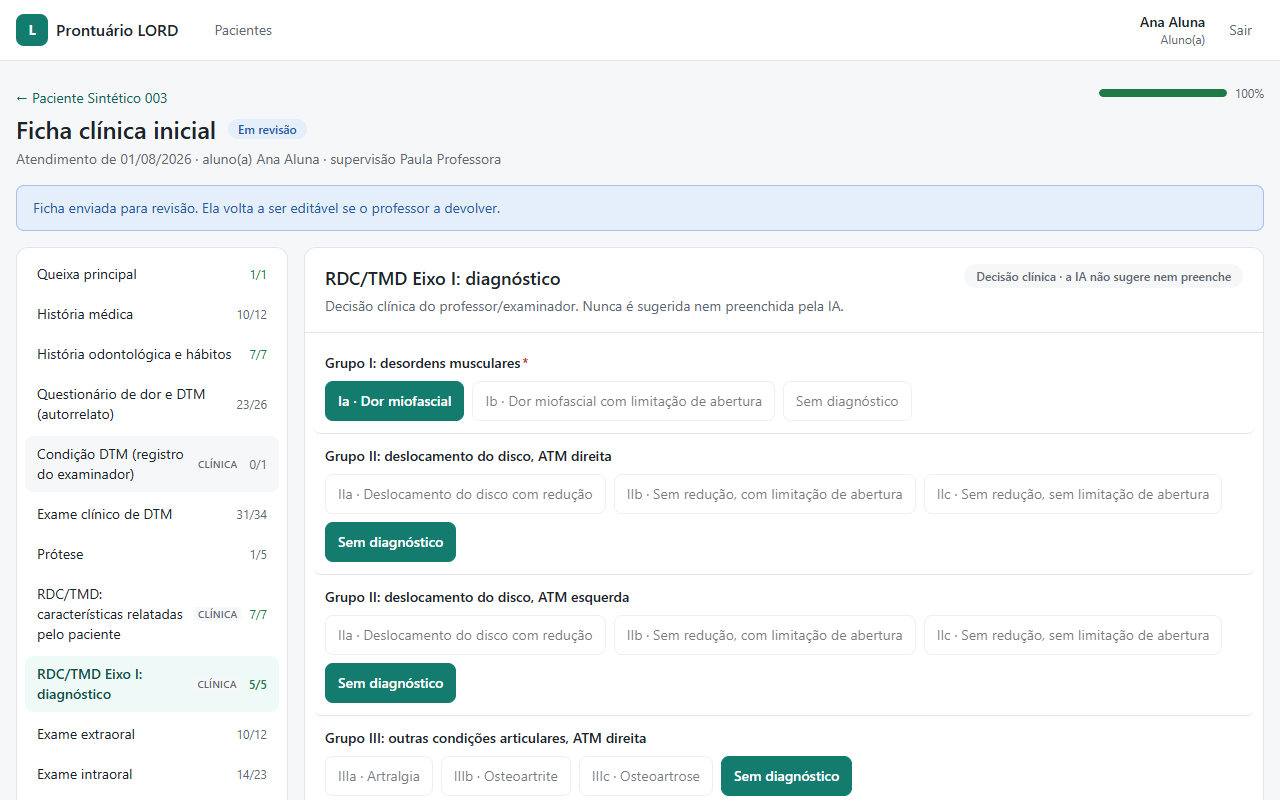
\includegraphics[width=\textwidth]{figuras/07-diagnostico-somente-humano}
	\fonte{Os autores (2026), com dados sintéticos.}
\end{figure}
\begin{figure}[htbp]
	\caption{Fila de revisão do professor}
	\label{fig:tela-revisao}
	\centering
	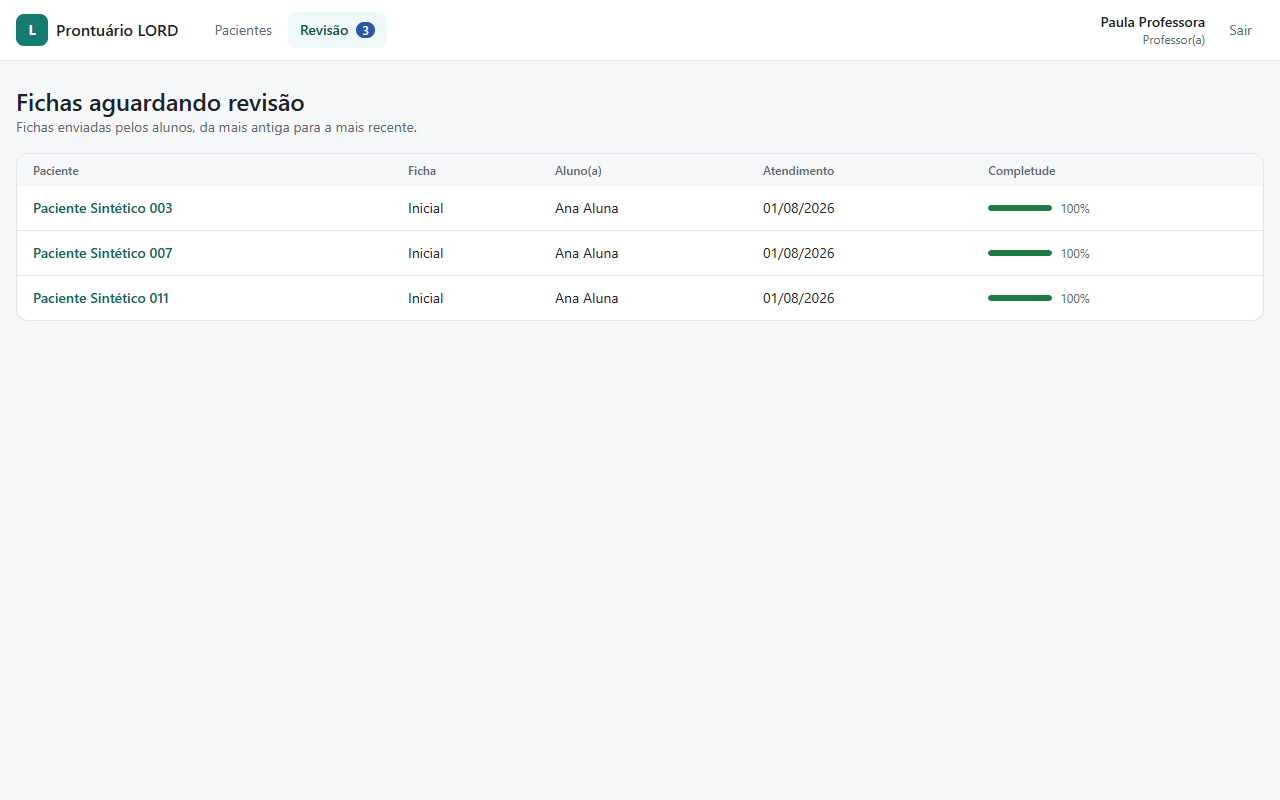
\includegraphics[width=\textwidth]{figuras/09-fila-revisao}
	\fonte{Os autores (2026), com dados sintéticos.}
\end{figure}

Nas seções que admitem ditado, a ficha exibe o painel ``Ditado com IA'' (\autoref{fig:tela-revisao-ia}). O acadêmico grava o relato, que é transcrito e pode ser corrigido antes do envio, ou digita o texto diretamente. As sugestões aparecem com o rótulo do campo, o valor proposto e, entre aspas, o trecho do relato que o justifica. Cada sugestão pode ser aceita ou rejeitada; ao aceitar, o valor é aplicado ao formulário, onde pode ser corrigido, e a decisão passa a constar como ``aceita e editada''. Quando a sugestão substituiria um valor já preenchido, o painel avisa e mostra o valor atual. Os valores descartados pelas salvaguardas ficam em uma lista recolhida, com o motivo do descarte. O painel não aparece nas seções exclusivamente humanas nem em fichas enviadas para revisão ou aprovadas.

\begin{figure}[htbp]
	\caption{Revisão das sugestões da IA com o trecho de evidência}
	\label{fig:tela-revisao-ia}
	\centering
	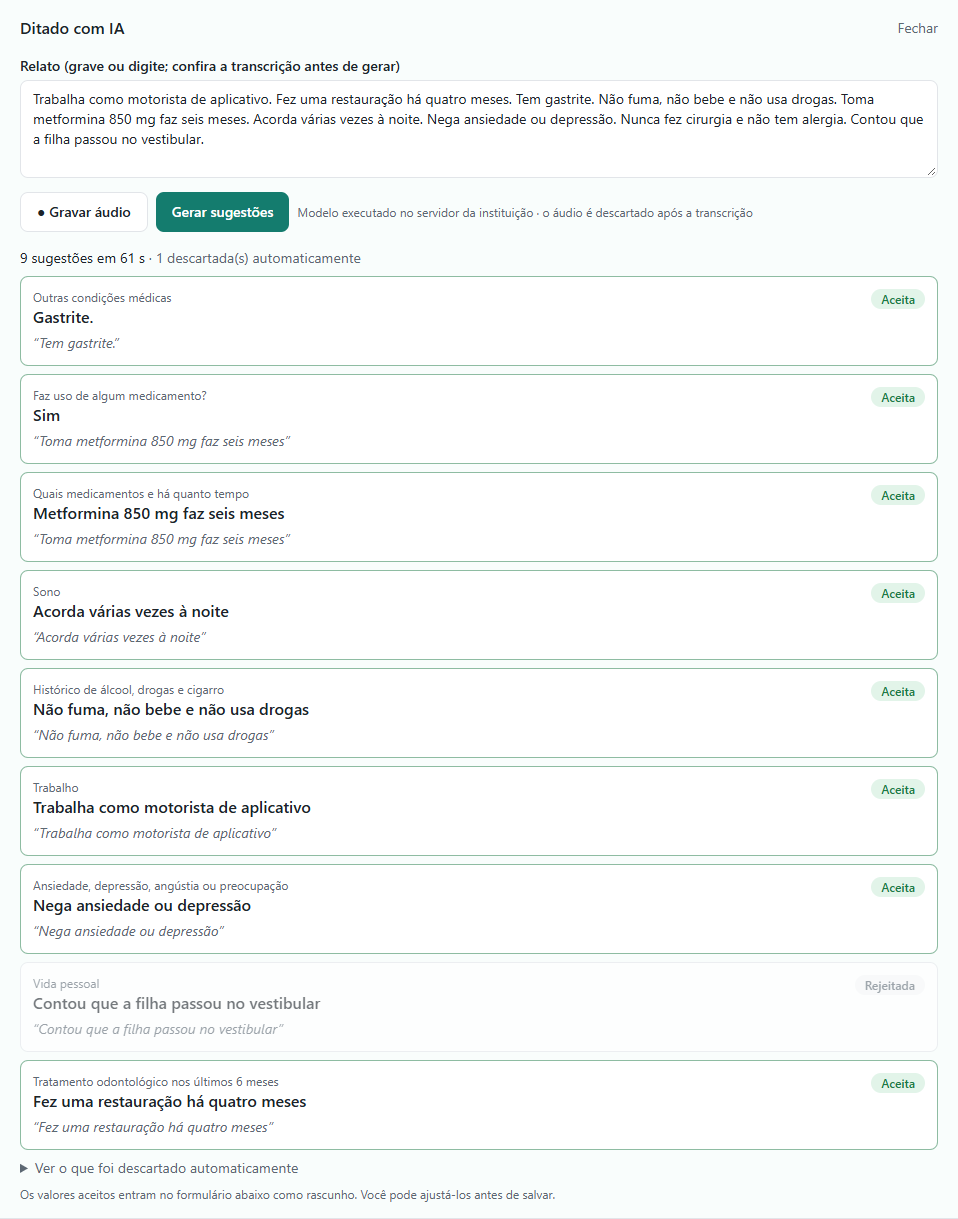
\includegraphics[width=0.85\textwidth]{figuras/11-revisao-ia}
	\fonte{Os autores (2026), com relato sintético e o modelo \texttt{qwen2.5:3b} (\textit{prompt} v4).}
\end{figure}

A \autoref{fig:tela-revisao-ia} foi gerada por um teste automatizado de ponta a ponta que executa o modelo real sobre um relato de desenvolvimento. O relato contém, de propósito, um comentário sem relação com a saúde (``a filha passou no vestibular''). O modelo o atribuiu ao campo ``vida pessoal'', com a citação correta, de modo que as salvaguardas não tinham como barrá-lo. O acadêmico o rejeitou na revisão, o que ilustra por que a revisão humana é obrigatória.

A latência é o principal limite do módulo no ambiente de desenvolvimento, um computador pessoal sem GPU: com o \texttt{qwen2.5:3b}, a estruturação de uma seção isolada pela interface levou de 35 a 104~s, e a das cinco seções que admitem ditado, de 1,3 a 3,8~minutos por relato de desenvolvimento, a uma taxa de cerca de 8~\textit{tokens} por segundo. A transcrição de 14,5~s de áudio pelo Whisper \texttt{small} levou 5,7~s, depois do carregamento inicial do modelo. \todo{medir a latência no servidor da UEPG, com e sem GPU.}

\begin{figure}[htbp]
	\caption{Painel de evolução clínica do paciente}
	\label{fig:tela-painel}
	\centering
	\figtodo{captura do painel do paciente, após a fase 5}
	\fonte{Os autores (2026).}
\end{figure}

\section{Avaliação técnica}

\begin{table}[htbp]
	\caption{Desempenho da persistência híbrida em comparação com o modelo normalizado}
	\label{tb:benchmark}
	\footnotesize
	\centering
	\begin{tabular}{|l|c|c|c|c|}
		\hline
		\multirow{2}{*}{\textbf{Métrica}} & \multicolumn{2}{c|}{\textbf{1.000 pacientes}} & \multicolumn{2}{c|}{\textbf{10.000 pacientes}} \\ \cline{2-5}
		& \textbf{JSONB} & \textbf{Normalizado} & \textbf{JSONB} & \textbf{Normalizado} \\ \hline
		Leitura do prontuário (ms) & -- & -- & -- & -- \\ \hline
		Escrita de um atendimento (ms) & -- & -- & -- & -- \\ \hline
		Espaço em disco (MB) & -- & -- & -- & -- \\ \hline
	\end{tabular}
	\fonte{Os autores (2026).}
\end{table}

Os requisitos de segurança e de integridade são verificados por testes automatizados. Os testes da API são de integração: cada execução cria um servidor PostgreSQL~17 descartável, aplica as migrações e exercita a API por requisições HTTP, verificando também o estado do banco diretamente. Os testes da interface usam a Testing Library para os componentes e o Playwright, com o navegador Microsoft Edge, para os fluxos de ponta a ponta. A \autoref{tb:testes} resume os 142 testes da versão atual. Nos testes do módulo de IA, o modelo de linguagem é substituído por um simulador que devolve respostas preparadas, o que torna os testes rápidos e determinísticos; um teste adicional, executado sob demanda, percorre o fluxo de ditado no navegador com o modelo real.

\begin{table}[htbp]
	\caption{Testes automatizados por componente}
	\label{tb:testes}
	\footnotesize
	\centering
	\begin{tabularx}{\textwidth}{|L{3.8cm}|Y|c|}
		\hline
		\textbf{Componente} & \textbf{O que é verificado} & \textbf{Testes} \\ \hline
		Esquema da ficha & Validade, cobertura das questões 1 a 75, esquema derivado para a IA, rótulos, campos condicionais, completude e salvaguardas da IA (evidência presente no relato, coerência entre valor e evidência, limpeza da citação) & 40 \\ \hline
		API: autenticação & Argon2id, \textit{cookie}, bloqueio, sessão, auditoria de acesso & 9 \\ \hline
		API: controle de acesso & Matriz de papéis na API e \textit{Row-Level Security} diretamente no banco & 10 \\ \hline
		API: pacientes & Cifragem dos dados pessoais, busca por CPF via HMAC, validação, auditoria & 6 \\ \hline
		API: fichas & Fluxo de revisão, imutabilidade, adendos, colunas geradas, odontograma & 7 \\ \hline
		API: esquema analítico & Isolamento do papel analítico, pseudônimos, ausência de textos livres & 5 \\ \hline
		API: sugestões da IA & Recusa de seções exclusivamente humanas e de fichas fora do rascunho, registro das sugestões e das decisões, falha do modelo, auditoria sem conteúdo & 7 \\ \hline
		Módulo de IA & Montagem do \textit{prompt}, formato de saída, descarte pelas salvaguardas (com modelo simulado), métricas e retomada do Experimento~A, distinção entre falha de conexão e saída inválida & 14 \\ \hline
		Serviço de transcrição & Idioma e vocabulário clínico enviados ao modelo, áudio mantido só em memória, recusa de arquivos que não são áudio, vazios, grandes demais ou ilegíveis & 6 \\ \hline
		Interface: componentes & Controle por tipo de campo, campos condicionais, erros, mapa de palpação, odontograma e painel de ditado (aceitar, rejeitar, aceitar todas, edição posterior) & 24 \\ \hline
		Interface: ponta a ponta & Fluxo completo da ficha no navegador (cadastro, preenchimento, persistência, revisão, aprovação) e restrição de telas por papel & 2 \\ \hline
		Gerador de casos sintéticos & Validade, reprodutibilidade, coerência clínica e compatibilidade com o sexo & 12 \\ \hline
		\textbf{Total} & & \textbf{142} \\ \hline
	\end{tabularx}
	\fonte{Os autores (2026).}
\end{table}

Entre as propriedades verificadas estão as seguintes. Um aluno não obtém, nem pela API nem por consulta direta com o papel da aplicação, os pacientes de outro aluno. O administrador não enxerga pacientes, embora consulte a auditoria. Nem o dono das tabelas consegue alterar ou excluir uma ficha aprovada. O texto original do CPF, do telefone e do endereço não aparece no valor gravado. O papel analítico não tem acesso às tabelas identificadas nem ao segredo dos pseudônimos, e as visões analíticas não contêm o nome do paciente nem trechos de texto livre.

\todo{resultado da varredura OWASP ZAP (alertas por severidade, antes e depois) e cobertura de testes.}

\section{Experimento A: qualidade da estruturação automática}

\begin{table}[htbp]
	\caption{Desempenho da estruturação automática no conjunto de teste}
	\label{tb:exp-a}
	\footnotesize
	\centering
	\begin{tabular}{|l|l|c|c|c|c|c|c|}
		\hline
		\textbf{Modelo} & \textbf{Estratégia} & \textbf{P} & \textbf{R} & \textbf{F1} & \textbf{Alucinação} & \textbf{Omissão} & \textbf{Latência (s)} \\ \hline
		Modelo 1 & Ficha inteira & -- & -- & -- & -- & -- & -- \\ \hline
		Modelo 1 & Por seção & -- & -- & -- & -- & -- & -- \\ \hline
		Modelo 2 & Ficha inteira & -- & -- & -- & -- & -- & -- \\ \hline
		Modelo 2 & Por seção & -- & -- & -- & -- & -- & -- \\ \hline
	\end{tabular}
	\fonte{Os autores (2026).}
\end{table}

\todo{F1 por seção da ficha (gráfico), validade estrutural, reprodutibilidade e análise qualitativa dos erros por categoria: negação, tempo, autocorreção, termos coloquiais.}

\section{Experimento B: captação por áudio versus texto}

\begin{table}[htbp]
	\caption{Taxa de erro de palavras e impacto na estruturação}
	\label{tb:exp-b}
	\footnotesize
	\centering
	\begin{tabular}{|l|l|c|c|c|}
		\hline
		\textbf{Modelo Whisper} & \textbf{Condição} & \textbf{WER geral} & \textbf{WER termos clínicos} & \textbf{$\Delta F_1$ vs. texto} \\ \hline
		\textit{small} & Silêncio & -- & -- & -- \\ \hline
		\textit{small} & Ruído & -- & -- & -- \\ \hline
		\textit{medium} & Silêncio & -- & -- & -- \\ \hline
		\textit{medium} & Ruído & -- & -- & -- \\ \hline
	\end{tabular}
	\fonte{Os autores (2026).}
\end{table}

\section{Experimento C: usabilidade e eficiência}

\todo{caracterização dos participantes (número, período do curso, experiência com a ficha).}

\begin{table}[htbp]
	\caption{Resultados por condição de registro}
	\label{tb:exp-c}
	\footnotesize
	\centering
	\begin{tabular}{|l|c|c|c|c|}
		\hline
		\textbf{Condição} & \textbf{Tempo (min)} & \textbf{Completude (\%)} & \textbf{Erros} & \textbf{NASA-TLX} \\ \hline
		Papel & -- & -- & -- & -- \\ \hline
		Formulário digital & -- & -- & -- & -- \\ \hline
		Formulário com ditado e IA & -- & -- & -- & -- \\ \hline
	\end{tabular}
	\fonte{Os autores (2026).}
\end{table}

\todo{escore SUS médio e intervalo de confiança; resultado do teste de Friedman; taxa de aceitação das sugestões; problemas de usabilidade por severidade; síntese das entrevistas.}

\section{Experimento D: validação do pipeline analítico}

\begin{table}[htbp]
	\caption{Efeitos programados e efeitos recuperados na coorte sintética}
	\label{tb:exp-d}
	\footnotesize
	\centering
	\begin{tabular}{|l|c|c|c|c|}
		\hline
		\textbf{Tratamento} & \textbf{Redução programada} & \textbf{Redução estimada} & \textbf{$p$ (Wilcoxon)} & \textbf{Redução $\geq$ 30\%} \\ \hline
		Placa oclusal & 40\% & -- & -- & -- \\ \hline
		Orientações & 10\% & -- & -- & -- \\ \hline
	\end{tabular}
	\fonte{Os autores (2026).}
\end{table}

\begin{figure}[htbp]
	\caption{Painel de coorte gerado a partir da coorte sintética}
	\label{fig:painel-coorte}
	\centering
	\figtodo{diagramas de caixa da variação da dor por tratamento e prevalência das características relatadas}
	\fonte{Os autores (2026).}
\end{figure}
